\documentclass[a4paper,14pt]{extarticle}

\usepackage{geometry}
\geometry{a4paper,tmargin=2cm,bmargin=2cm,lmargin=3cm,rmargin=1cm}
\usepackage[T2A]{fontenc}
\usepackage[utf8]{inputenc}
\usepackage[english,main=russian]{babel}
\usepackage{indentfirst}
\usepackage{graphicx}
\graphicspath{{./images/}}
\usepackage{setspace}
\linespread{1.3}
\usepackage{tempora}
\usepackage{amsmath}
\usepackage{booktabs}
\usepackage{array}
\usepackage{caption}
\usepackage{hyperref}
\hypersetup{unicode=true,hidelinks}
\usepackage{listings}

\sloppy
\clubpenalty=10000
\widowpenalty=10000



\lstset{basicstyle=\ttfamily\small,breaklines=true,
  columns=fullflexible,frame=single,numbers=none,
  showstringspaces=false,tabsize=4,captionpos=t,keepspaces=true}
\renewcommand{\lstlistingname}{Листинг}
\begin{document}

\begin{titlepage}
\thispagestyle{empty}

\vspace*{-60pt}

\hspace*{-82pt}
\begin{minipage}{0.3\textwidth}
\centering
\IfFileExists{images/emblem.png}{%
  
\includegraphics[width=0.9\textwidth]{emblem.png}%
}{%
  \IfFileExists{images/emblem.jpg}{%
    \includegraphics[width=0.9\textwidth]{emblem.jpg}%
  }{}%
}
\end{minipage}
\begin{minipage}{0.67\textwidth}
\small
\textbf{
\vspace*{-0.7ex}
\centerline{Министерство науки и высшего образования Российской Федерации}
\vspace*{-0.7ex}
\centerline{Федеральное государственное бюджетное образовательное учреждение}
\vspace*{-0.7ex}
\centerline{высшего образования}
\vspace*{-0.7ex}
\centerline{<<Московский государственный технический университет}
\vspace*{-0.7ex}
\centerline{имени Н. Э. Баумана}
\vspace*{-0.7ex}
\centerline{(национальный исследовательский университет)>>}
\vspace*{-0.7ex}
\centerline{(МГТУ им. Н. Э. Баумана)}
}
\end{minipage}

\vspace{-25pt}
\hspace{-35pt}\rule{\textwidth}{2.3pt}

\vspace*{-20.3pt}
\hspace{-35pt}\rule{\textwidth}{0.4pt}

\vspace{1.5ex}
\hspace{-35pt}\noindent\small
ФАКУЛЬТЕТ\hspace{80pt} <<Информатика и системы управления>>

\vspace*{-16pt}
\hspace{47pt}\rule{0.83\textwidth}{0.4pt}

\vspace{0.5ex}
\hspace{-35pt}\noindent\small
КАФЕДРА\hspace{50pt} <<Теоретическая информатика и компьютерные технологии>>

\vspace*{-16pt}
\hspace{30pt}\rule{0.866\textwidth}{0.4pt}

\vspace{11em}

\begin{center}
\Large \textbf{Лабораторная работа №2} \\
\large \textbf{по курсу <<Параллельные и распределённые системы>>} \\
\large <<Параллельное решение системы линейных алгебраических уравнений>>
\end{center}

\normalsize

\vspace{8em}

\begin{flushright}
Студент группы ИУ9-51Б \\
Шалимов Д. И. \\
\vspace{2ex}
Преподаватель Царев А.С.
\end{flushright}

\bigskip
\vfill

\begin{center}
\textsl{Москва 2026}
\end{center}
\end{titlepage}

\setcounter{page}{2}
\tableofcontents
\newpage



\section{Постановка задачи и метод решения}
Цель работы --- реализовать решение СЛАУ $Ax=b$ методом простой итерации
с использованием OpenMP и MPI и сравнить производительность реализаций.
Вычисления выполняются в типе \texttt{double}. В модельной матрице
на диагонали стоят двойки, вне диагонали --- единицы.
Для основного эксперимента точное решение $u_i=1$, правая часть $b_i=N+1$,
начальное приближение $x^{(0)}=0$.

На каждой итерации вычисляется невязка и при необходимости обновляется решение:
\[
 r^{(k)}=Ax^{(k)}-b,\qquad
 x^{(k+1)}=x^{(k)}-\tau r^{(k)},\qquad \tau=\frac{0.1}{N}.
\]
Критерий остановки --- $\|r^{(k)}\|_2/\|b\|_2<\varepsilon$.
Проверка выполняется до обновления $x$.
Матрица положительно определена; её максимальное собственное значение равно
$N+1$. Выбранный шаг удовлетворяет условию сходимости $0<\tau<2/(N+1)$.
В программе используется обычное плотное умножение матрицы на вектор,
без упрощения вычислений за счёт специального вида матрицы.

\section{Реализация}
В \texttt{solver\_openmp.c} матрица и векторы находятся в общей памяти.
Функция \texttt{multiply} распределяет строки между потоками;
каждый поток записывает свой элемент результата. В \texttt{dot}
сумма для нормы невязки вычисляется через \texttt{reduction(+:sum)}.
Неявные барьеры отделяют вычисление невязки от обновления решения.

\begin{lstlisting}[language=C,caption={Распределение строк в OpenMP}]
#pragma omp parallel for schedule(static)
for (int i = 0; i < n; ++i) {
    double sum = 0.0;
    for (int j = 0; j < n; ++j)
        sum += a[(size_t)i * n + j] * x[j];
    result[i] = sum;
}
\end{lstlisting}

В \texttt{solver\_mpi.c} каждый процесс хранит последовательный блок строк
матрицы и полные векторы $x$ и $b$. Функция \texttt{make\_layout} задаёт
размеры блоков и смещения; число строк у процессов отличается не более
чем на одну. Функция \texttt{multiply\_local} считает локальную невязку,
а \texttt{MPI\_Allreduce} суммирует её квадраты на всех процессах.
После обновления локальных частей новый $x$ собирается у каждого участника:

\begin{lstlisting}[language=C,caption={Сборка полного вектора в MPI}]
MPI_Allgatherv(new_x, local_rows, MPI_DOUBLE,
               x, counts, offsets, MPI_DOUBLE,
               MPI_COMM_WORLD);
\end{lstlisting}

Таймер охватывает только итерационное решение; подготовка данных и проверка
ответа не учитываются. В MPI перед измерением вызывается
\texttt{MPI\_Barrier}, а итоговое время --- максимум локальных времён,
полученный через \texttt{MPI\_Reduce} с \texttt{MPI\_MAX}.
Подробный разбор функций и директив вынесен в отдельный файл
\texttt{DEFENSE.md}; полные исходники приложены к работе отдельно.

\section{Результаты и анализ}
Использованы сохранённые измерения для $N=16000$, $\varepsilon=10^{-12}$,
режима \texttt{known} при 1, 2, 4, 8 и 16 работниках.
Устройство: Intel Core i5-13500H, 12 физических ядер и 16 логических
процессоров, 16~ГБ ОЗУ, Windows~11. Компиляция --- с \texttt{-O2}.
Для каждого сочетания выполнен один запуск.

Ускорение $S(p)=T(1)/T(p)$ и эффективность $E(p)=S(p)/p$ рассчитаны
относительно собственного однопоточного или однопроцессного запуска
каждой реализации. Время приведено в секундах.

\begin{table}[htbp]\centering
\caption{Измеренное время, ускорение и эффективность}
\small
\setlength{\tabcolsep}{5pt}
\begin{tabular}{r rrr rrr}
\toprule
 & \multicolumn{3}{c}{MPI} & \multicolumn{3}{c}{OpenMP} \\
\cmidrule(lr){2-4}\cmidrule(lr){5-7}
$p$ & $T$ & $S$ & $E$ & $T$ & $S$ & $E$ \\
\midrule
1 & 139.038 & 1.000 & 1.000 & 140.619 & 1.000 & 1.000 \\
2 & 76.578 & 1.816 & 0.908 & 70.205 & 2.003 & 1.001 \\
4 & 42.343 & 3.284 & 0.821 & 42.754 & 3.289 & 0.822 \\
8 & 16.688 & 8.332 & 1.041 & 24.983 & 5.629 & 0.704 \\
16 & 16.415 & 8.470 & 0.529 & 15.671 & 8.973 & 0.561 \\
\bottomrule
\end{tabular}
\end{table}

Все десять запусков завершились со сходимостью за 263 обновления.
Относительная невязка составила $4.639824613892\cdot10^{-13}$,
максимальная ошибка решения --- $8.618661340165\cdot10^{-13}$.
На рисунке~\ref{fig:performance} показаны зависимости от числа работников.

В этой серии минимальное время получено при 16 работниках:
16.415114~с для MPI и 15.670640~с для OpenMP.
У MPI переход от 8 к 16 процессам дал лишь небольшое улучшение,
у OpenMP выигрыш оказался заметнее.
Значение $E>1$ при восьми процессах MPI относится к единичному замеру
и не доказывает устойчивого сверхлинейного ускорения. На результат могли
влиять кэш, частота процессора и фоновая нагрузка; отдельно они не измерялись.

\begin{figure}[p]\centering
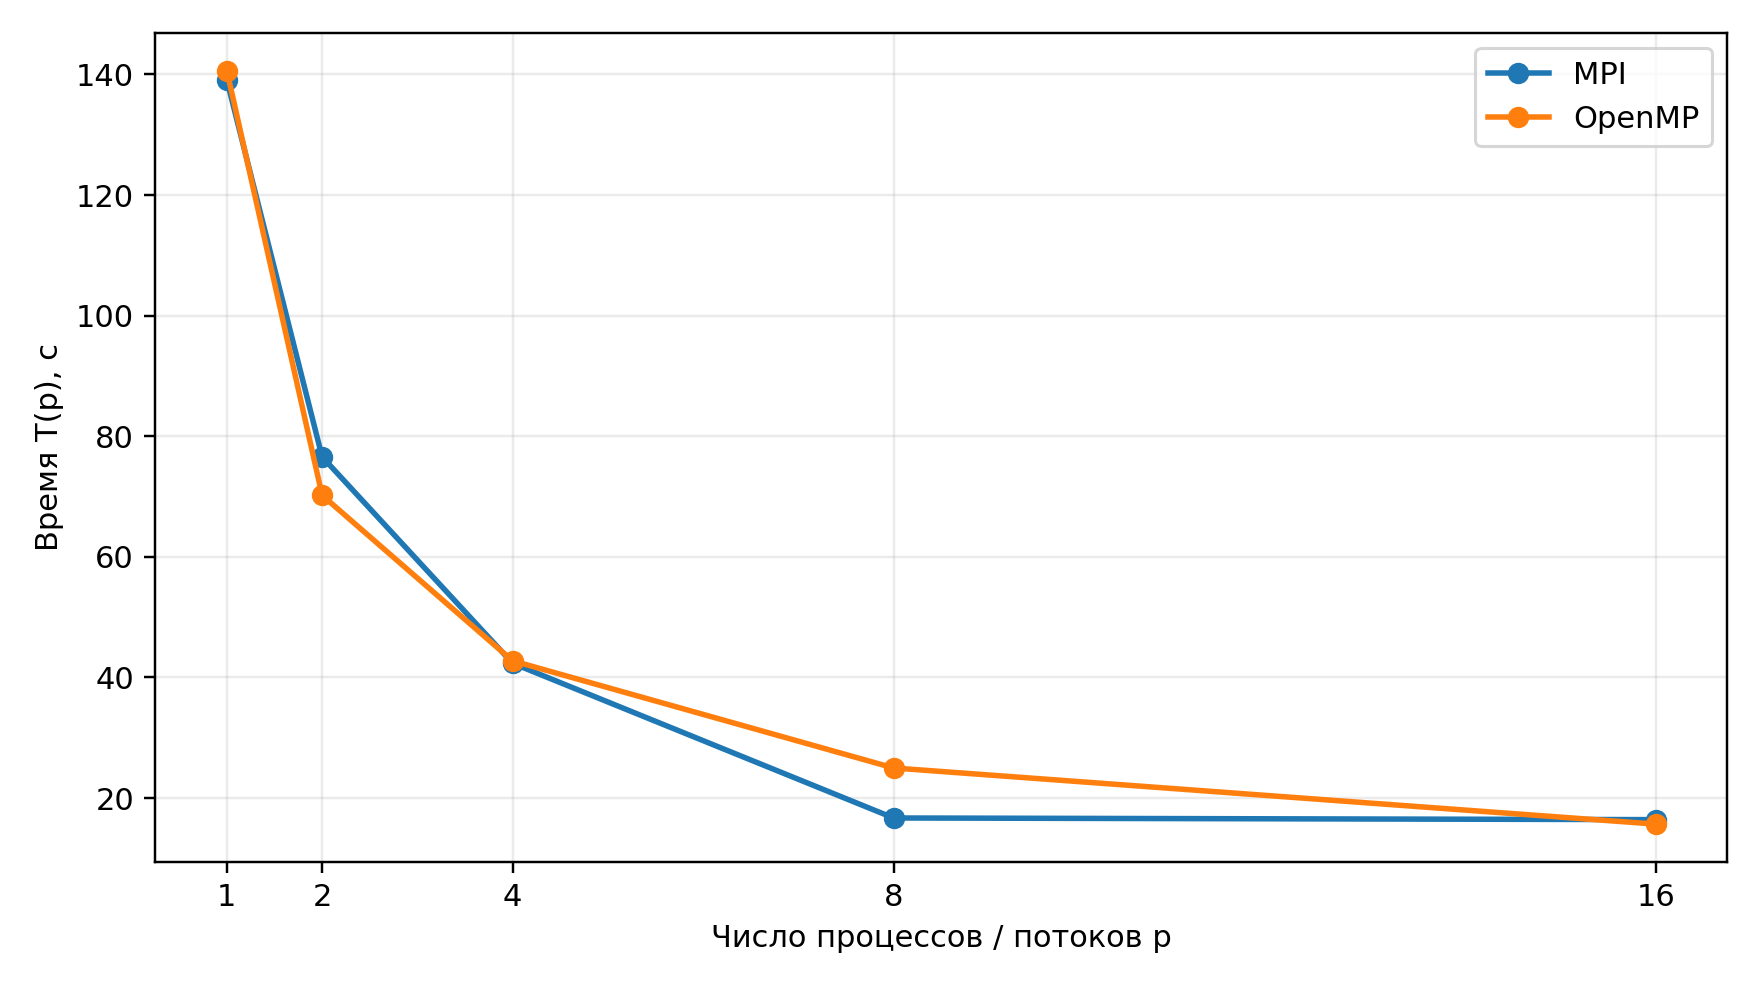
\includegraphics[width=0.85\textwidth,height=0.23\textheight,keepaspectratio]{lab2_time.png}\par\medskip
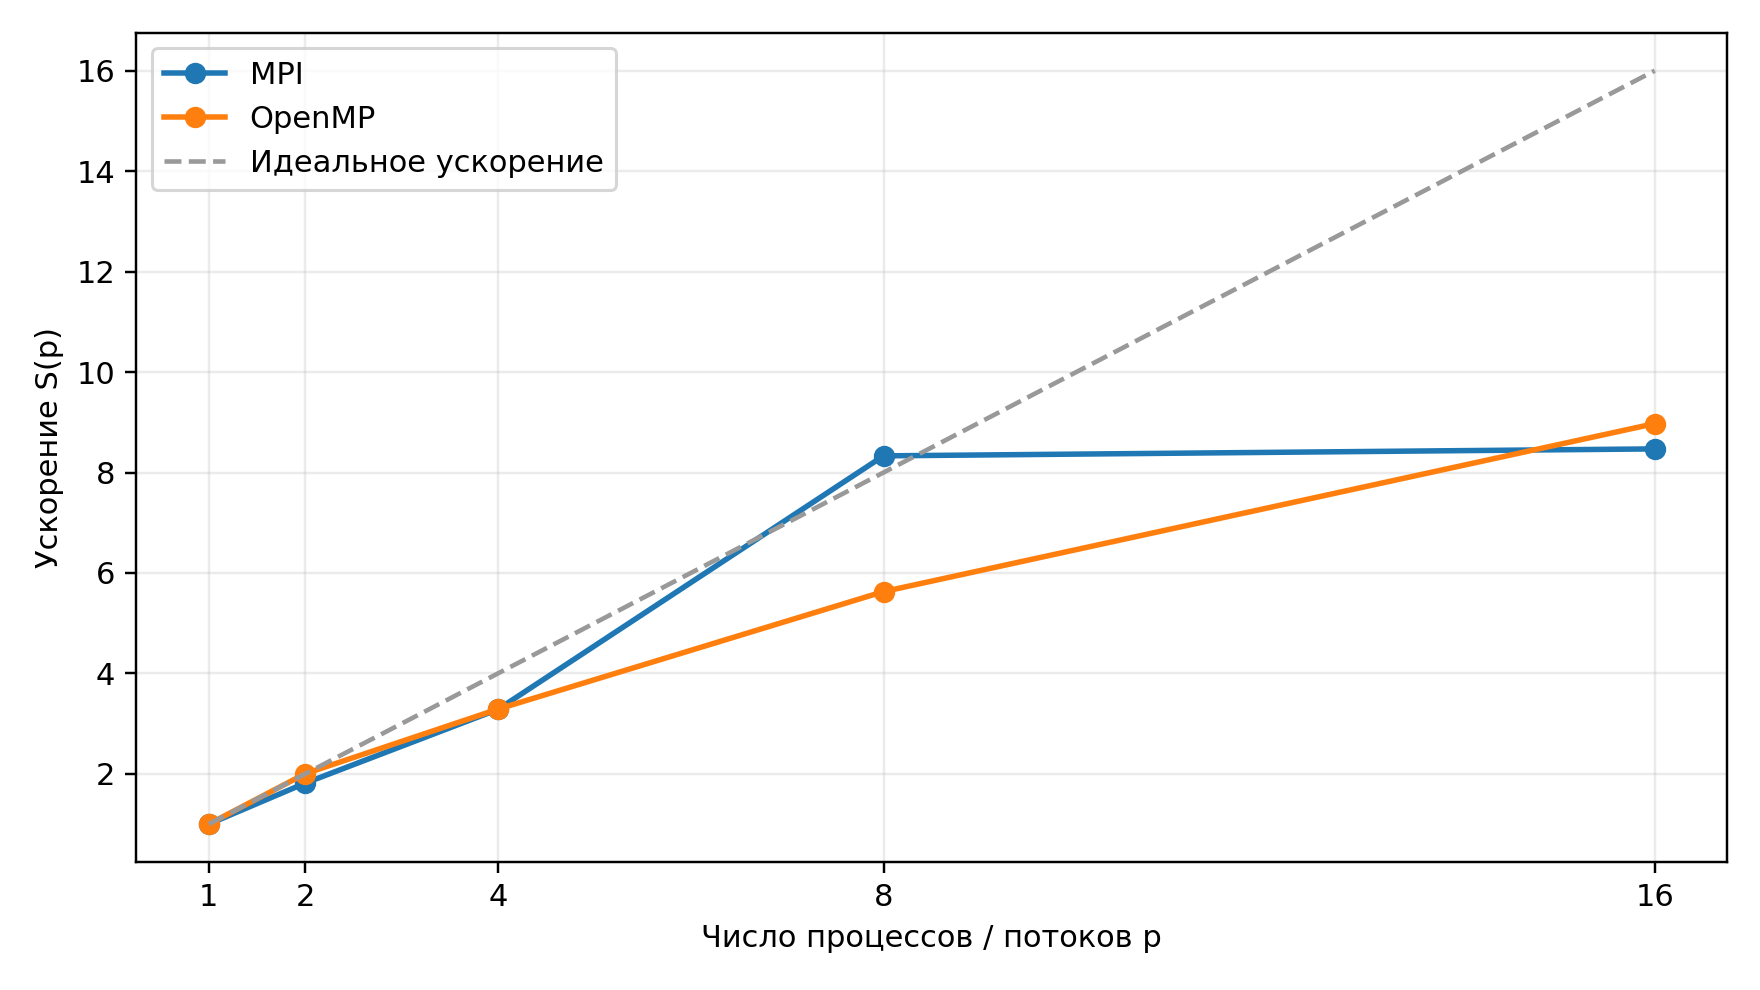
\includegraphics[width=0.85\textwidth,height=0.23\textheight,keepaspectratio]{lab2_speedup.png}\par\medskip
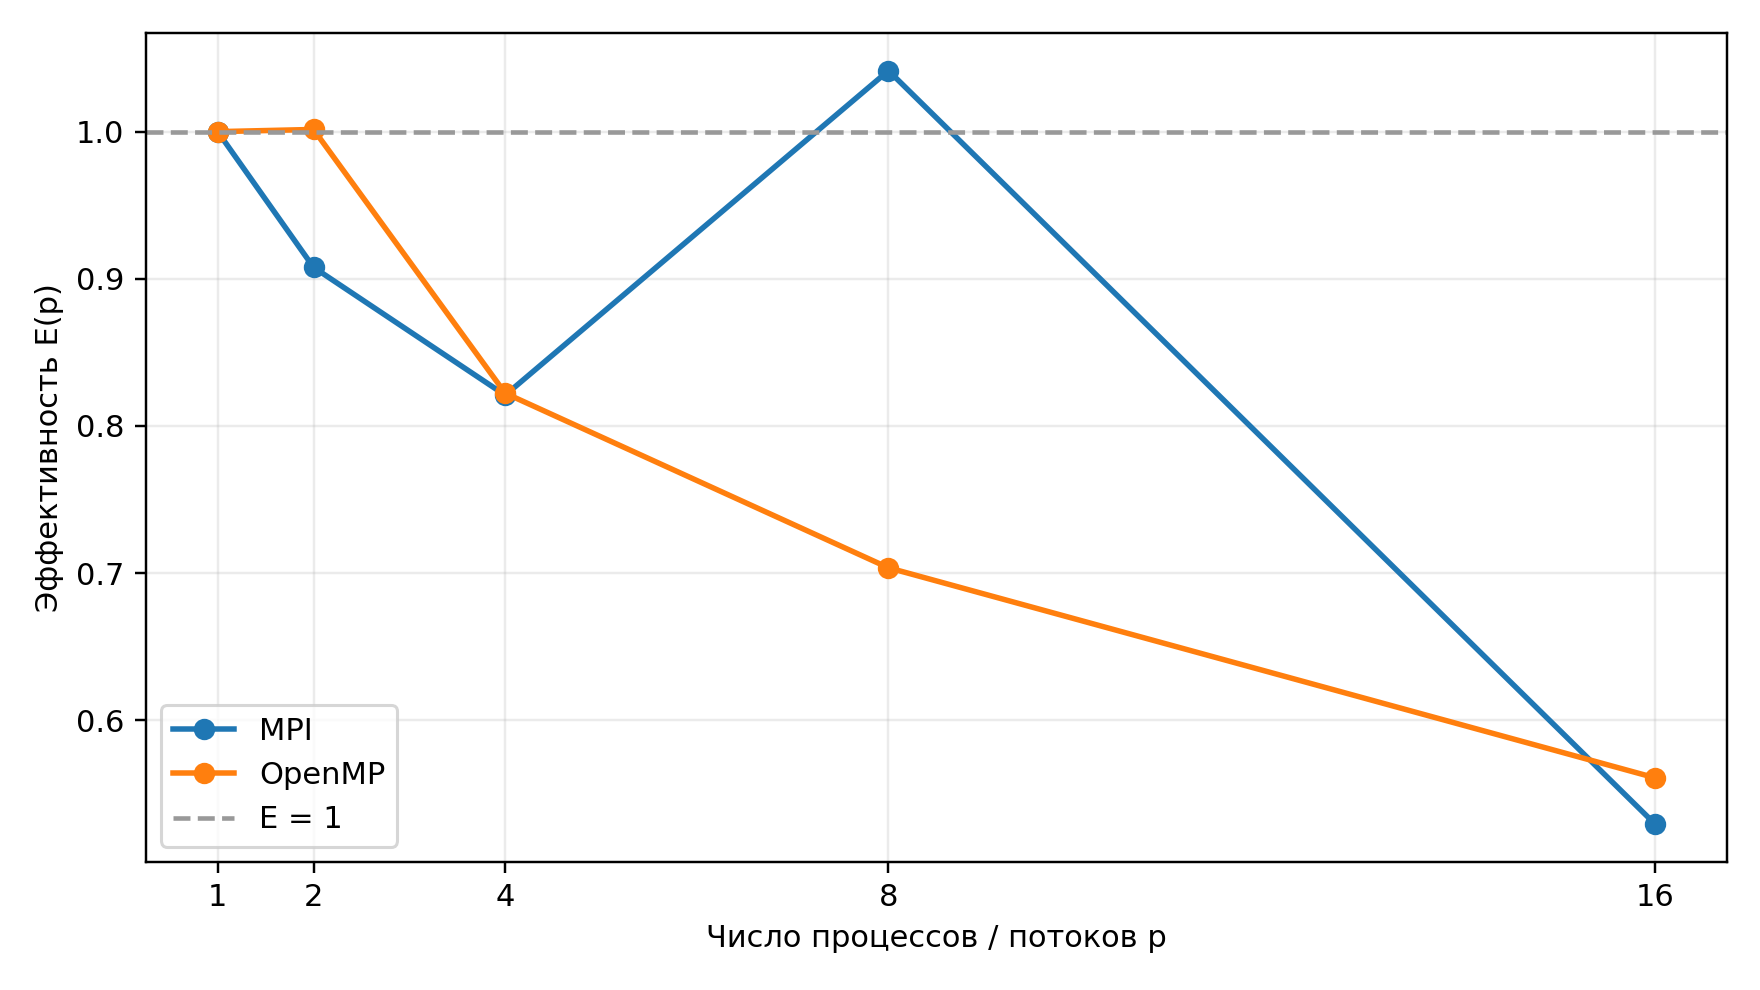
\includegraphics[width=0.85\textwidth,height=0.23\textheight,keepaspectratio]{lab2_efficiency.png}
\caption{Время, ускорение и эффективность MPI и OpenMP}
\label{fig:performance}
\end{figure}
\section{Вывод}
Реализованы две параллельные версии метода простой итерации с одинаковой
численной задачей. OpenMP использует общую память и распределяет строки
между потоками, MPI хранит строки в разных процессах и явно обменивается
данными. Корректность подтверждена невязкой и сравнением с известным решением.
Максимальное ускорение в сохранённой серии составило 8.470 для MPI и
8.973 для OpenMP. Результаты показывают выигрыш от распараллеливания,
но выводы о стабильности ускорения требуют повторных измерений.

\end{document}
